\chapter{Basic Techniques}
\label{ch:design::basics}

\begin{preamble}
This chapter covers two basic algorithm-design techniques: reduction and brute force.
\end{preamble}

\section{Algorithmic Reduction}
\label{sec:design::reduction}

\begin{definition}[Algorithmic Reduction]
\label{def:design::reduction}
We say that a problem~$A$ is \defn{reducable} to another problem~$B$,
if any instance of~$A$ can be reduced to one or more instances of~$B$.
%
This means that it is possible to solve any instance of~$A$ by
following the a three step process (also illustrated below).
%
\begin{itemize}
\item Transform the instance of problem~$A$ to one or many instances of problem~$B$.
\item Solve all instances of problem~$B$.
\item Use results to $B$ instances to compute result to
 the $A$ instance.
\end{itemize}
%
We sometimes refer to problem~$B$ as a \defn{subproblem} of~$A$,
especially if the reduction involves producing multiple instances
of~$B$.
%

\begin{center}
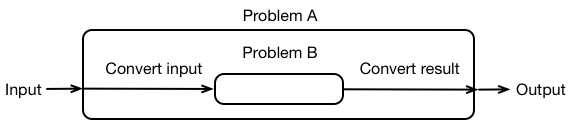
\includegraphics[width=5in]{./design/media-basics/reduction.jpg}
\end{center}

\end{definition}


%% \begin{definition}[Efficient Reduction]
%% \label{def:design::reduction::efficient}
%% We say that an reduction is efficient if the cost of two
%% transformations (of he input and the result) do not contribute
%% significantly to the cost.
%% %
%% More precisely, a reduction of $A$ to $B$ is~\defn{ (asymptotically)
%%   efficient}~if the transformations take asymptotically no more work
%% or span than $B$ on the same input size as $A$.
%% %
%% Thus an efficient reduction of problem $A$ to problem $B$ tells us
%% that problem $A$ is as easy as problem $B$.
%% \end{definition}

\begin{gram}[Efficiency of Reduction]
\label{gr:design::reduction::efficiency}

The efficiency of an algorithm obtained via reduction depends on the
complexity of the problem being reduced to, and the cost of
transforming the instances and putting together the results to compute
final result.
%
It is therefore important to ensure that the costs of the instance
transformation and the cost of computing the final result remain small in
comparison to the cost of the problem being reduced to.

We generally think of a reduction as being~\defn{efficient} if the
total cost of the input and output transformations are asymptotically
the same as that of the problem being reduced to.
%
\end{gram}

\begin{example}[Reduction from Maximal to Sorting]
  We can reduce the problem of finding the maximal element in a
  sequence to the problem of (comparison) sorting.
%
To this end, we sort the sequence in ascending order and then select
the last element, which is one the largest elements in the input
sequence.  
%

In this reduction, we don't need to transform the input.
%
To compute the final result, we retrieve the last element in the
sequence, which usually requires logarithmic work or less.
%
Because comparison sorting itself requires $\Theta(n\lg{n})$ work for
a sequence of $n$ elements, the reduction is efficient.
%
But, the resulting algorithm is not a work-efficient: it requires
$\Theta(n\lg{n})$ work, whereas we can find the maximum element of a
sequence in $\Theta(n)$ work.
\end{example}

\begin{example}[Reduction from Minimal to Maximal]
Suppose that we wish to find the minimal element in a sequence but
only know how to find the maximal element efficiently in linear work.
%
We can reduce the minimality problem to the maximality problem by
inverting the sign of all the elements in the input, finding the
maximal value of the transformed input, and then inverting the sign of
the result to obtain the minimum.
%
Because these computations require linear work in the size of the
input sequence, and because finding the maximal element requires
linear work, this reduction is quite efficient.
%

The resulting algorithm, which requires linear work in total, is also
asymptotically work efficient.
\end{example}

\begin{remark}
Reduction is a powerful technique and can allow us to solve a problem
by reducing it to another problem, which might appear very different
or even unrelated.
%
For example, we might be able to reduce a problem on strings such as
that of finding the shortest superstring of a set of strings to a
graph problem.
%
We have seen \href{sec:genome::alg}{an example of this earlier in genome sequencing.}
%
\end{remark}

\begin{remark}[Proving Hardness by Reduction]
Reduction technique can also be used ``in the other direction'' to
show that some problem is at least as hard as another or to establish
a lower bound.
%
In particular, if we know (or conjecture) that problem $A$ is hard
(e.g., requires exponential work), and we can reduce it to problem $B$
(e.g., using polynomial work), then we know that $B$ must also be
hard. 
%
Such reductions are central to the study of complexity theory.
\end{remark}


\section{Brute Force}
\label{sec:design::bf}

\begin{gram}
The brute-force technique involves enumerating all possible solutions,
a.k.a.,~\defn{candidate solutions} to a problem, and checking whether
each candidate solution is valid.
%
Depending on the problem, a solution may be returned as soon as it is
found, or the search may continue until a better solution is found.
\end{gram}

\begin{example}[Brute-Force Sorting]
We are asked to sort a set of keys $a$.
%
As a first algorithm, we can apply the brute force technique by
considering the candidate-solution space (sequence of keys),
enumerating this space by considering each candidate, and checking
that it is sorted. 

More precisely speaking, this amounts to trying all permutations
of~$a$ and testing that each permutation is sorted. 
%
We return as soon as we find a sorted permutation.
%
Because there are $n!$ permutations and $n!$ is very large even
for small $n$, this algorithm is inefficient.
%
For example, using Sterling's approximation, 
we know that  $100! \approx \frac{100}{e}^{100} \ge 10^{100}$.
%
There are only about $10^{80}$ atoms in the universe so there is
probably no feasible way we could apply the brute force method
directly.
%
We conclude that this approach to sorting is
not~\defn{tractable}, because it would require a lot of energy and time for all but  tiny inputs.
\end{example}

%
\begin{remark}
The total number of atoms in the (known) universe, which is less than
$10^{100}$ is a good number to remember.
%
If your solution requires this much work or time, it is probably
intractable.
\end{remark}
%

\begin{important}
Brute-force algorithms are usually naturally parallel.
%
Enumerating all candidate solutions (e.g., all permutations, all
elements in a sequence) is typically easy to do in parallel and so is
testing that a candidate solution is indeed a valid solution.
%
But
brute-force algorithms are usually not work efficient and therefore not desirable---in algorithm design, our first priority
is to minimize the total work and only then the span.
\end{important}

\begin{teachask}
  Can you suggest a brute-force algorithm for finding the largest
  element in a sequence.  What is the complexity?
\end{teachask}
%
\begin{example}[Maximal Element]
Suppose that we are given a sequences of natural numbers and we wish
to find the maximal number in the sequence.
%
To apply the brute force technique, we first identify the solution
space, which consists of the elements of the input sequence.
%
The brute-force technique advises uses to try all candidate solutions.
%
We thus pick each element and test that it is greater or equal to all
the other elements in the sequence.  When we find one such element, we
know that we have found the maximal element.
%

This algorithm requires $\Theta(n^2)$ comparisons and can be effective
for very small inputs, but it is far from an optimal algorithm, which
would perform $\Theta(n)$ comparisons.  .
\end{example}

%% \begin{question}
%% Does the brute-force technique parallelize well?
%% \end{question}
%

%% \begin{question}
%% Given that the brute-force algorithms are often inefficient, why do we
%% care about them?
%% \end{question}


\begin{example}[Brute-Force Overlaps]
\label{ex:design::bf::overlaps}
  Given two strings $a$ and $b$, let's define the
  (maximum)~\defn{overlap} between $a$ and $b$ as the largest suffix
  of $a$ that is also a prefix of $b$. For example, the overlap
  between ``15210'' and ``2105'' is ``210'', and the overlap between
  ``15210'' and ``1021'' is ``10''.
%

We can find the overlap between~$a$ and~$b$ by using the brute force
technique.
%
We first note that the solution space consists of the suffixes of~$a$
that are also prefixes of~$b$.
%
To apply brute force, we consider each possible suffix of~$a$ and
check if it is a prefix of~$b$.
%
We then select the longest such suffix of~$a$ that is also a prefix
of~$b$.
%

The work of this algorithm is $|a| \cdot |b|$, i.e., the product of
the lengths of the strings. 
%
Because we can try all positions in
parallel, the span is determined by the span of checking that a particular prefix is also a suffix, which is $O(\lg{|b|})$.  
%
Selecting the maximum requires  $O(\lg{|a|})$ span.
%
Thus the total span is $O(\lg{(|a| + |b|)})$.

\end{example}


\begin{exercise}
The analysis given in the \href{ex:design::bf::overlaps}{example above} is not ``tight'' in the sense that there is a bound that is asymptotically dominated by
$O(|a| \cdot |b|)$.  
%
Can you improve on the bound? 
%% Tight bound is $O(min(a,b)^2)$.
\end{exercise}


\begin{example}[Brute-Force Shortest Paths]
\label{ex:design::bf::shortest-paths}
Consider the following problem: we are given a graph where each edge
is assigned distance (e.g., a nonnegative real number), and asked to find
the shortest path between two given vertices in the graph.

Using brute-force, we can solve this problem by enumerating the
solution space, which is the set of all paths between the given two
vertices, and selecting the path with the smallest total distance.
%
To compute the total distance over the path, we sum up the distances
of all edges on the path.
\end{example}


\begin{example}[Brute-Force Shortest Distances]
\label{ex:design::bf::shortest-distances}
Consider the following variant of the shortest path problem: we are
given a graph where each edge is assigned a distance
%
(e.g., a nonnegative real number), 
%
and asked to find the shortest distance between two given vertices in
the graph.  This problem differs from the one above, because it asks
for the shortest distance rather than the path.
%

Using brute-force, we might want to solve this problem by enumerating
the solution set, which is the real numbers starting from zero, and
selecting the smallest one.
%
But, this is impossible, because real numbers are not countable, and
cannot be enumerated.
%

One solution is to use the \href{sec:design::reduction}{reduction technique}
and reduce the problem to the shortest-path version of the problem \href{ex:design::bf::shortest-paths}{described above} and then compute the distance of the returned path.
%

As an additional refinement, we can reformulate \href{ex:design::bf::shortest-paths}{the shortest-path problem} to return the distance of the shortest path in addition to the path itself.  
%
With this refinement, computing the final result requires no
additional computation beyond returning the distance.
%
\end{example}


\begin{important}[Strengthening]
We used an important technique in
\href{ex:design::bf::shortest-distances}{the shortest-paths example} where we refined the problem that we are reducing to so that it returns us more information than strictly necessary.  
%
This technique is called \defn{strengthening} and is commonly employed
to improve efficiency by reducing redundancy.
\end{important}

\begin{example}[Brute-Force Shortest Paths (Decision Version)]
\label{ex:design::bf::shortest-paths-decision}
Consider the ``decision problem'' variant of the shortest path
problem: we are given a graph where each edge is assigned a distance
(e.g., a nonnegative real number), and we are given a \defn{budget},
which is a distance value.
%
We are asked to check whether there is a path between two given
vertices in the graph that is shorter than the given budget.  
%
This problem differs from the shortest path problem, because it asks
us to return a ``Yes'' or ``No'' answer. Such problems are
called~\defn{decision problems}.

Using brute force, we could enumerate all candidate
solutions, which are either ``Yes'' or ``No'', and test whether each
one is indeed a valid solution.
%
In this case, this does not help, because we are back to our original
problem that we started with.
%
Again, we can ``refine'' our brute-force approach a bit by reducing it
to the original \href{ex:design::bf::shortest-paths}{shortest-path problem}, and then checking whether the distance of the resulting path is larger than the budget.
%
\end{example}

\begin{remark}
Experienced algorithms designers  perform reductions between
different variants of the problem as shown in the last two examples
``quietly'' (\exref{design::bf::shortest-distances} and
\exref{design::bf::shortest-paths-decision}).
%
That is, they don't explicitly state the reduction but simply apply
the brute-force technique to a slightly different set of candidate
solutions.
%
For beginners and even for experienced designers, however, recognizing
such reductions can be instructive.
\end{remark}

\begin{remark}[Utility of Brute Force]
Even though brute-force algorithms are usually inefficient, they can
be useful.
%
\begin{itemize}
\item Brute-force algorithms are usually easy to design and are a good starting point toward a more efficient algorithm.  They can help in   understanding the structure of the problem, and lead to a more efficient algorithm.

\item In practice, a brute-force algorithm can help in testing the correctness of   a more efficient algorithm by offering a solution that is easy to implement correctly.
%


\end{itemize}
\end{remark}

%% \begin{checkpoint}

%% \begin{questionfr}
%% \points 10

%% \prompt
%% Describe a brute-force algorithm for deciding whether an integer $n$
%% is composite (not prime).   

%% \answer

%% \end{questionfr}
%% \end{checkpoint}

